\documentclass[12pt,a4,english,finnish,pdflatex%,handout
]{beamer}
\definecolor{MyGreen}{RGB}{50, 120, 50}
\usecolortheme[named=MyGreen]{structure}

\usepackage{babel}
\usepackage[utf8]{inputenc}
\usepackage[T1]{fontenc}
\usepackage{amsmath,amssymb} 
\usepackage{animate}
\usepackage{multimedia}

\usepackage{natbib}
\bibpunct[: ]{(}{)}{,}{}{}{;}

\usepackage{tikz}

\usepackage{tipa}

\usepackage{hyperref}

\setbeamertemplate{navigation symbols}{}

\graphicspath{{figures/}}

\setlength{\leftmargini}{0pt}
\setlength{\leftmarginii}{1em}

%% Write out the names of graphics files being included 
\newwrite\graphics
\immediate\openout\graphics=\jobname.graphics%
\let\oincludegraphics\includegraphics% store original \includegraphics
\renewcommand{\includegraphics}[2][]{% prepend to it (could also use xpatch, etc.)
  \immediate\write\graphics{#2}
  \oincludegraphics[#1]{#2}}

\newcommand\Wider[2][3em]{%
\makebox[\linewidth][c]{%
  \begin{minipage}{\dimexpr\textwidth+#1\relax}
  \raggedright#2
  \end{minipage}%
  }%
}

\newcommand{\kommentti}[1]{
  {\bf[#1]}
}


\title{CSD 598 - Winter 2026
  \\~\\
  Getting started and Epistemology
}
\author{Pertti Palo and Shanda Duggleby Wenzel} 
\date{13 Jan 2026} 


\begin{document}

\frame{\titlepage
  \centering
} 

\frame{\frametitle{Land acknowledgement}

The University of Alberta, its buildings, labs and research stations are
primarily located on the territory of the Néhiyaw (Cree), Niitsitapi
(Blackfoot), Métis, Nakoda (Stoney), Dene, Haudenosaunee (Iroquois) and
Anishinaabe (Ojibway/ Saulteaux), lands that are now known as part of Treaties
6, 7 and 8 and homeland of the Métis. The University of Alberta respects the
sovereignty, lands, histories, languages, knowledge systems and cultures of all
First Nations, Métis and Inuit nations. 

}

\frame{\frametitle{Other preliminaries}
\begin{itemize}
  \item "The most important thing in our lives".
  \item Thank you for your gift of time.
\end{itemize}
}

\frame{\frametitle{Who are these people?}
  \begin{columns}
    \begin{column}{5cm}
      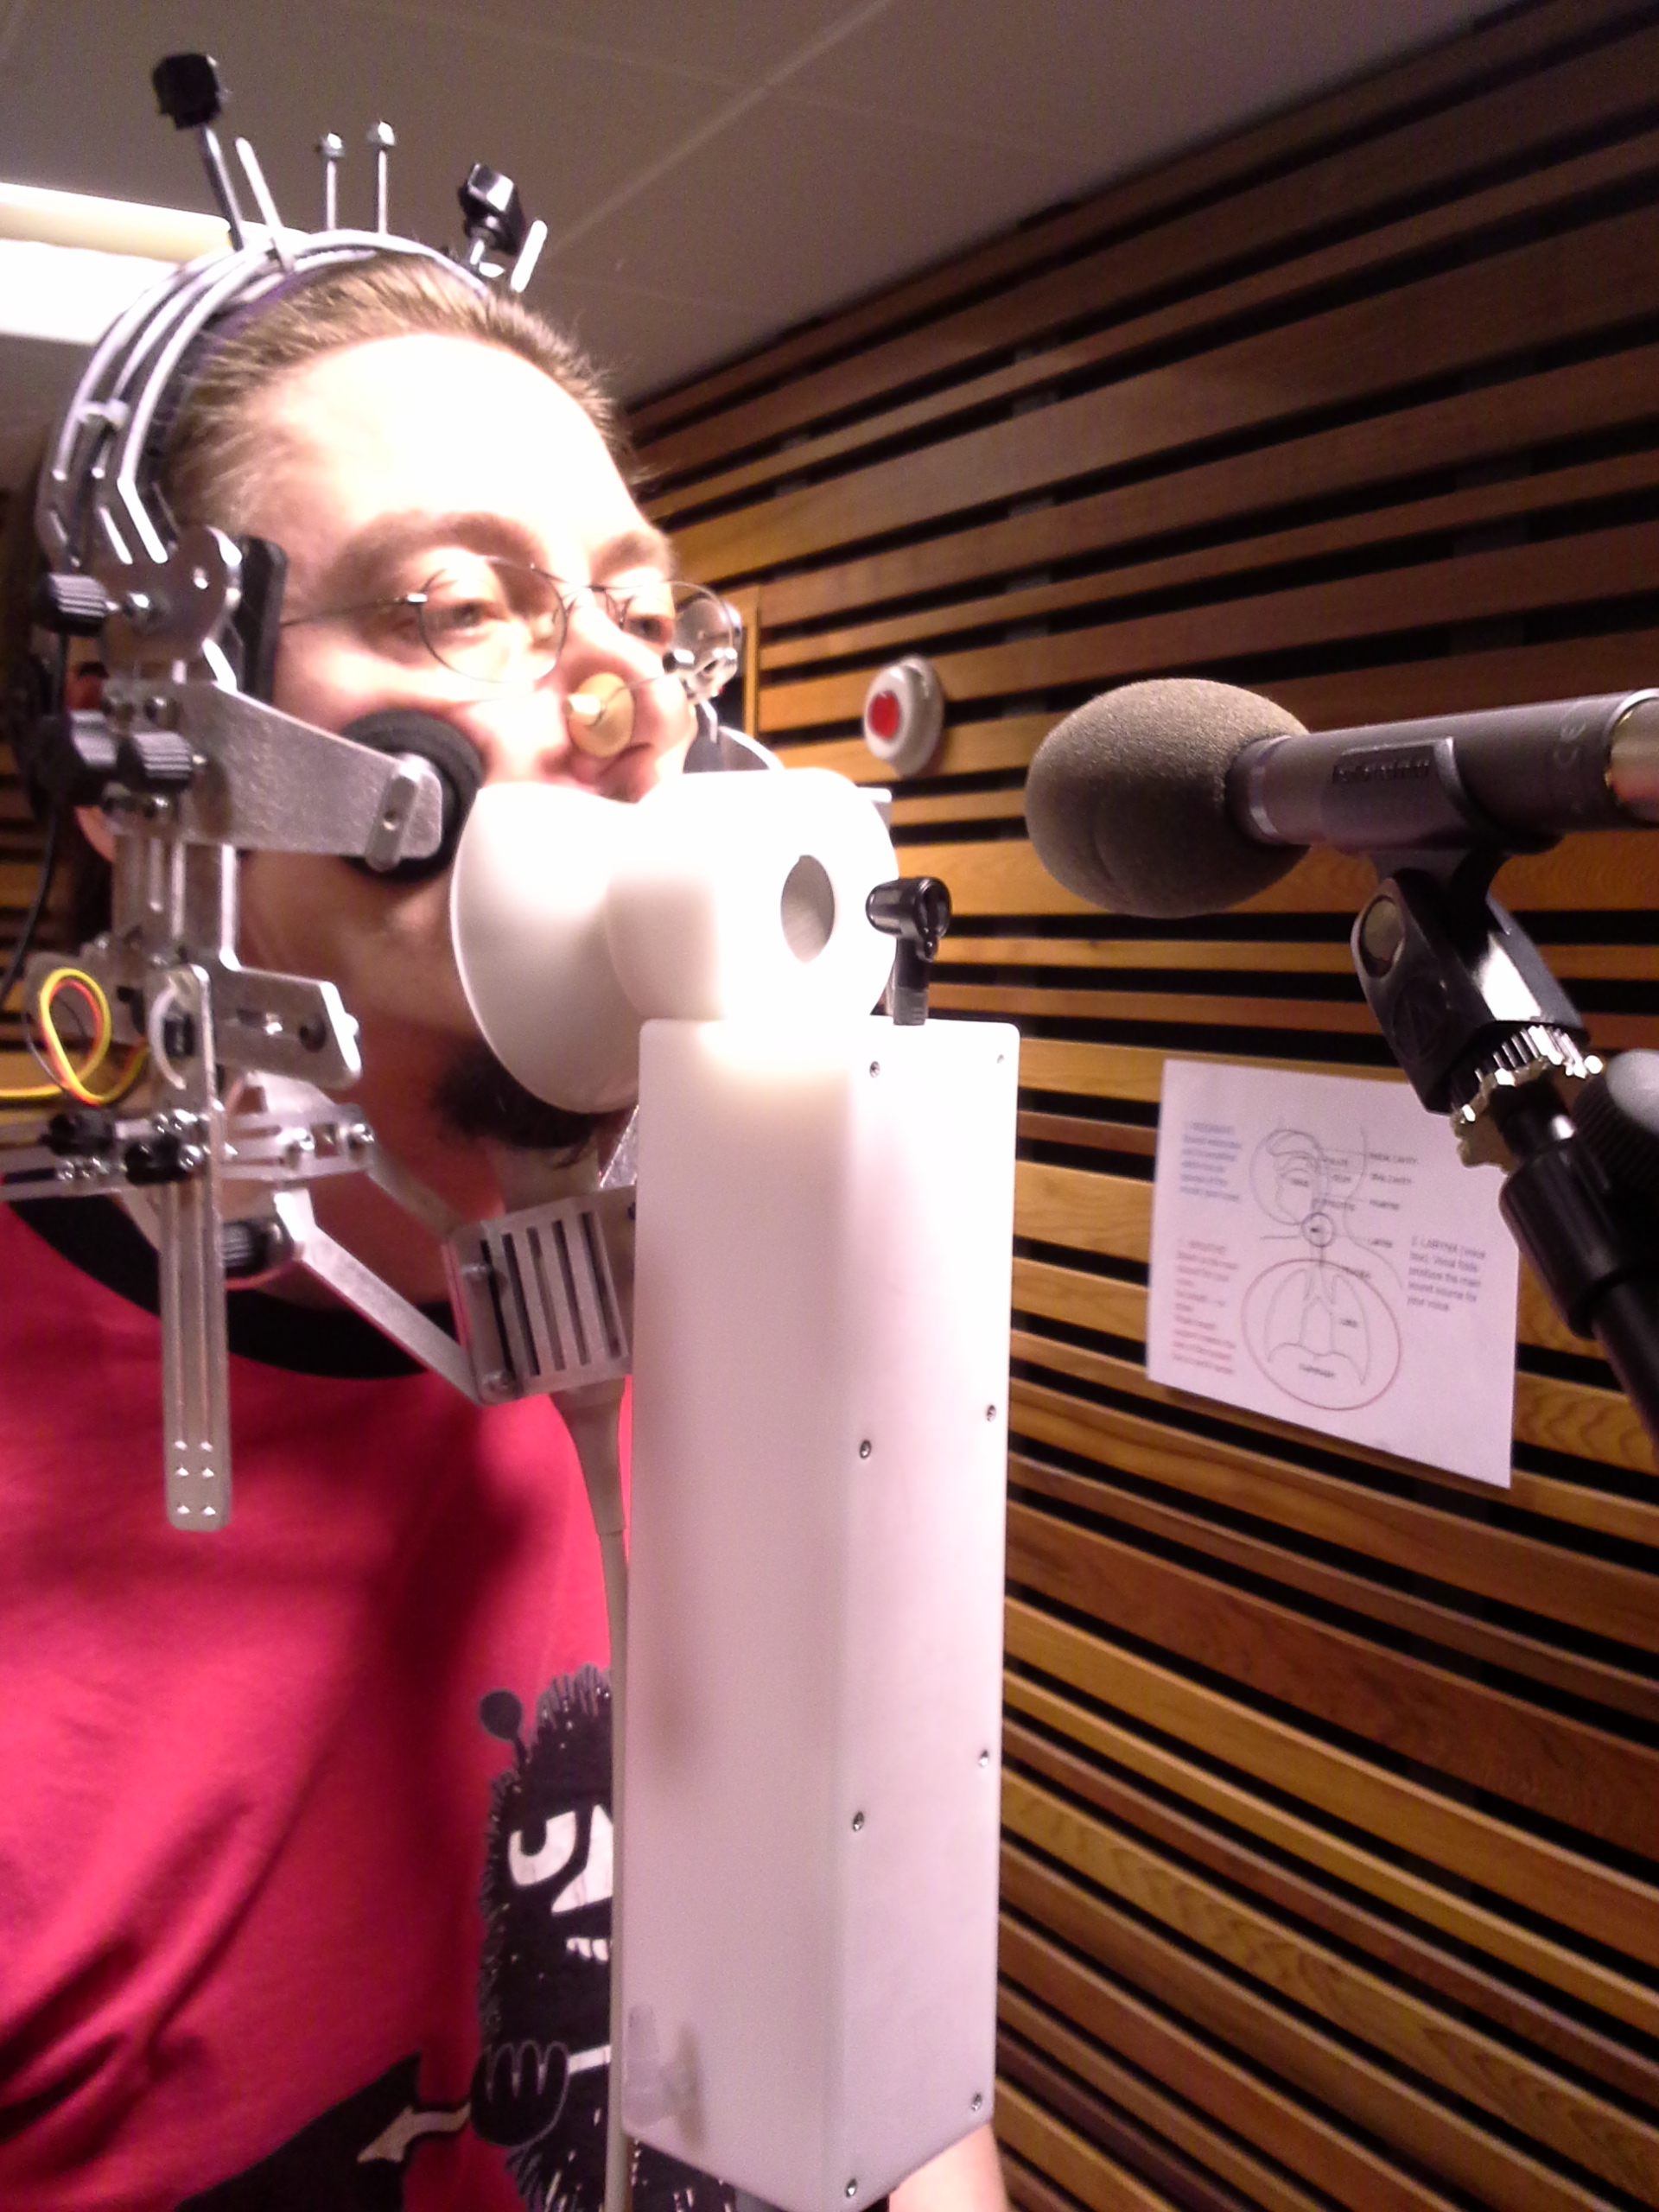
\includegraphics[width=\columnwidth]{uti_eva.png}
    \end{column}
    \begin{column}{5cm}
      \begin{itemize}
      \item Pertti Palo
      \item I have a Masters engineering, a Licentiate in maths, and a PhD in
      Phonetics.
      \item I speak fluent phonetician, engineer, mathematician, and
      statistician.
      \item My super power is quantitative methods: both recording and
      analysis.
      \end{itemize}
    \end{column}
  \end{columns}
} 


\frame{\frametitle{Who are you then?}
  \begin{itemize}
  \item What's your name?
  \item What's your relevant background?
  \item What brings you here?
  \item What is your thing in life?
  \end{itemize}
} 


\frame{
  \centering
  {
    \bf \Large 
    \usebeamercolor[fg]{title}
    Let's plan the course together
    
    \vfill
%    \includegraphics[height=1.5cm]{figures/aalto_logo} 
  }
}


\frame{\frametitle{Tentative schedule, part 1}

These are all subject to changing depending on your input.

\begin{description}
  \item[13th Jan] This is today. We'll go through how the course works and talk a bit about epistemology.
  \item[20th Jan] Data exploration: descriptive statistics and data visualisation.
  \item[27th Jan] Speed run of CSD 501.
  \item[3rd Feb] Reporting statistics, potential pitfalls of methods from 501.
  \item[10th Feb] Linear mixed models and how all models are (kinda) the same model.
  \item[17th Feb] Reading week. No lecture.
  \item[24th Feb] Bayesian statistics and how our tools guide our questions.     
\end{description}
}


\frame{\frametitle{Tentative schedule, part 2}

These are all subject to changing depending on your input.

\begin{description}
  \item[3rd Mar] qualitative research 
  \item[10th Mar] qualitative research 
  \item[17th Mar] transformative paradigm
  \item[24th Mar] practical suggestions, e.g., organizing yourself for research
  \item[31st Mar] practical suggestions, e.g., preparing and submitting an ethics 
  \item[7th Apr] summary / catch up / other 
  \item[Possible other topics] speed run of other fun stats tools including AI,
  data and analysis planning, what to do with bad data, can data be too good,
  inter-rater issues.
\end{description}
}


\frame{\frametitle{How to pass this course with flying colours}

\Wider{
  These (also) are all subject to changing depending on your input.
  \vspace{.5cm}

  Short reflection essays.
  \begin{description}
    \item[Jan 20, by end of] Reflection on your expectations and goals for the course. 
    \item[Feb 24, by end of] Reflection on quantitative research 
    \item[Mar 31, by end of] Reflection on qualitative/transformative research
  \end{description}
  Consider rubric from CSD 505. Whichever one you do best is the one that counts as your grade.
  \vspace{.5cm}

  Critical evaluation of an article.
  \begin{description}
    \item[Apr 7, by end of] Either you pick or we pick. (Ours will be short.)
  \end{description}
  }
}


\frame{\frametitle{Learning outcomes}
\begin{itemize}
  \item What do we want them to be?
\end{itemize}
}


\frame{
  \centering
  {
    \bf \Large 
    \usebeamercolor[fg]{title}
    An important note on notes
    
    \vfill
%    \includegraphics[height=1.5cm]{figures/aalto_logo} 
  }
}

\frame{\frametitle{Note on note taking}
\begin{itemize}
  \item It's a good idea to keep a record of your developing understanding and
  especially of the questions you have.
  \item It's also a good idea to keep a record of any anomalies (or lack
  thereof) in data gathering because that makes analysis easier.
  \item Notebooks are good and there are way more possibilities out there
  beyond a regular composition notebook, which is a very solid choice though.
  \item Knowledge management systems such as Obsidian, Notion, Logseq and
  others can also be very useful, but might be more difficult and distracting
  to use during data recording.
  \item These also apply to this and any other course, which is why this topic
  is here. 
\end{itemize}
}


\frame{
  \centering
  {
    \bf \Large 
    \usebeamercolor[fg]{title}
    Epistemology and Ontology
    
    \vfill
%    \includegraphics[height=1.5cm]{figures/aalto_logo} 
  }
}


\frame{\frametitle{Definitions - one take}
\Wider{
  \begin{description}[\leftmargin=20pt]
    \item[Epistemology] "is the branch of philosophy that examines the nature,
    origin, and limits of knowledge. [\ldots] Epistemologists study the
    concepts of belief, truth, and justification to understand the nature of
    knowledge. To discover how knowledge arises, they investigate sources of
    justification, such as perception, introspection, memory, reason, and
    testimony."
    \item[Ontology] "is the philosophical study of being. [\ldots] To articulate
    the basic structure of being, ontology examines the commonalities among all
    things and investigates their classification into basic types, such as the
    categories of particulars and universals. [\ldots] Systems of categories aim
    to provide a comprehensive inventory of reality by employing categories such
    as substance, property, relation, state of affairs, and event."
  \end{description}
  See \cite{Wikipedia-Epistemology-2025,Wikipedia-Ontology-2026}
  }
}

\frame{\frametitle{Causality}
\begin{itemize}
  \item We all know - or should know - by now that correlation does not imply causation.
  \item But what is causality?
  \begin{itemize}
    \item David Hume has said that causality can not be proven empirically because we can not know if the world changes at a fundamental level.
    \item Immanuel Kant has replied to this that causality is not a feature of the universe, but rather a way or tool of reasoning.
    \item In addition, some phenomena in quantum physics break causality empirically. And in the general theory of relativity we can not say what the order of two events occurring is because it depends on the point of observation.
    \item And this could all be wrong, but it's unlikely (or seems unlikely given the evidence).
  \end{itemize}
  \item Unless this was not news, it should make one think. And that's what I'd like to encourage in any case.
\end{itemize}
}

\frame{\frametitle{Causality and other tools}
\begin{itemize}
  \item It is not enough to know how to use a tool, we should also understand enough of its workings that we know
  \begin{itemize}
    \item the limits of our understanding
    \item the limits of the tool
  \end{itemize}
  \item Statistics is a tool. Like causality.
\end{itemize}
}


\frame{\frametitle{Questions and thoughts to keep you thinking}
\begin{itemize}
  \item What do we assume to be true when using statistics?
  \item What do we assume to be true when doing empirical research?
  \item Does (can) one experiment refute generations of knowledge?
  \item Science is (also) an oral tradition. 
  \item Science relies heavily on (somewhat formalised) storytelling.
\end{itemize}
}

\frame{\frametitle{References}
  
\bibliographystyle{apalike}
\bibliography{science_combined}

}
\end{document}

